\documentclass[cjk,slidestop,compress,mathserif,blue]{beamer}
%dvipdfm选项是关键,否则编译统统通不过
%beamer的颜色选项定义的是导航条和标题的颜色(即关键词structure的颜色)

%%%%%%%%%%%%%%%%仅限于XeTeX可使用的宏包%%%%%%%%%%%%%%%%%%%%%%%%%%%%
\usepackage{fontspec,xunicode,xltxtra,beamerthemesplit}
%\usepackage{beamerthemesplit}
\usepackage{xeCJK}
\setCJKmainfont[BoldFont=黑体, ItalicFont=楷体, BoldItalicFont=仿宋]{黑体}
%\setsansfont[Mapping=tex-text]{Adobe 黑体 Std}
%如果装了Adobe Acrobat,可在font.conf中配置Adobe字体的路径以使用其中文字体
%也可直接使用系统中的中文字体如SimSun,SimHei,微软雅黑 等
%原来beamer用的字体是sans family;注意Mapping的大小写,不能写错

%%%%%%%%   确定标题和导航条结构的框架     %%%%%%%%%%%%
\usepackage{beamerthemeshadow}                       %
%\usepackage{beamerthemeclassic}%导航条色与背景色一致%
%%%%%%%%%%%%%%%%%%%%%%%%%%%%%%%%%%%%%%%%%%%%%%%%%%%%%%
\setbeamerfont{roman title}{size={}}
%\usepackage{CJK} % CJK 中文支持                                  %
\usepackage{amsmath,amsthm,amsfonts,amssymb,bm}
\usepackage{mathrsfs}
\usepackage{xcolor}                                        %使用默认允许使用颜色
\usepackage{hyperref} 
\usepackage{graphicx}
\usepackage{subfigure}           %图片跨页

%\usepackage[numbers,sort&compress]{natbib} %紧密排列             %
\usepackage[sectionbib]{chapterbib}        %每章节单独参考文献   %
\usepackage{hypernat}                                                                         %
%\usepackage[dvipdfm,bookmarksopen=true,pdfstartview=FitH,CJKbookmarks]{hyperref}		%
\hypersetup{bookmarksnumbered,colorlinks,linkcolor=brown,citecolor=blue,urlcolor=red}         %
%参考文献含有超链接引用时需要下列宏包,注意与natbib有冲突        %
%\usepackage[dvipdfm]{hyperref}                                  %
%\usepackage{hypernat}                                           %
\newcommand{\upcite}[1]{\hspace{0ex}\textsuperscript{\cite{#1}}} %

%\useoutertheme{smoothbars}
\useinnertheme[shadow=true]{rounded}
\usetheme{Berkeley}                                          %主题式样
%\usetheme{Luebeck}

\usecolortheme{lily}                                        %颜色主题式样

\usefonttheme{professionalfonts}                           %字体主题样式宏包

%\beamertemplatetransparentcoveredhigh                      %使所有被隐藏的文本高度透明
\beamertemplatetransparentcovereddynamicmedium             %使所有被隐藏的文本完全透明,动态,动态的范围很小
\mode<presentation>
%\beamersetaveragebackground{gray}                          %设置背景颜色(单一色) 
\beamertemplateshadingbackground{green!10}{red!5}         %设置背景颜色(渐变色)

%在指定位置精确放置logo
\usepackage{tikz}
\usepackage{beamerfoils}
\usepackage{pgf}
\logo{\pgfputat{\pgfxy(11.68,0.15)}{
\includegraphics[height=1.01cm,viewport=0 0 140 120,clip]{Figures/BCC_logo-1.png}}\pgfputat{\pgfxy(10.502,-0.218)}{
\includegraphics[height=0.369cm,viewport=140 0 540 120,clip]{Figures/BCC_logo-1.png}}}
%\logo{\pgfputat{\pgfxy(11.68,0.15)}{
\includegraphics[height=0.95cm,viewport=0 0 510 360,clip]{Figures/Logo_Gainstrong.png}}\pgfputat{\pgfxy(10.333,-0.195)}{
\includegraphics[height=0.35cm,viewport=530 70 1100 218,clip]{Figures/Logo_Gainstrong.png}}}
%\MyLogo{
%	\pgfputat{\pgfxy(-50,-50)}{\pgfbox[right,base]{
\includegraphics[height=1cm]{Figures/BCC_logo-1.png}}}

%logo作为背景放置
%\setbeamertemplate{background}{
%	\pgfputat{\pgfxy(6.5,-0.5)}{\pgfbox[left,top]{\pgfimage[height=1.1cm]{Figures/BCC_logo-1.png}}}}

%\logo{}									%不显示logo

\begin{document}
%\begin{CJK*}{GBK}{song}
%\begin{CJK*}{GBK}{kai}
%beamer下不能用\songyi、\zihao等命令!
%\graphicspath{Figures/}

%-------------------------------PPT Title-------------------------------------
\title{k空间布点与积分(一)}
%-----------------------------------------------------------------------------

%----------------------------Author & Date------------------------------------
\author{北京市计算中心\;云平台\:姜骏}
\date{\textrm{2016.11.09}}
%\date{2013.09.10}
\frame{\titlepage}
%-----------------------------------------------------------------------------

%------------------------------------------------------------------------------列出全文 outline ---------------------------------------------------------------------------------
\section*{}
\frame[allowframebreaks]
{
  \frametitle{Outline}
%  \frametitle{\textcolor{mycolor}{\secname}}
  \tableofcontents%[current,currentsection,currentsubsection]
}
%在每个section之前列出全部Outline
%类似的在每个subsection之前列出全部Outline是\AtBeginSubsection[]
\AtBeginSection[]
{
  \frame<handout:0>
  {
    \frametitle{Outline}
%全部Outline中,本部分加亮
    \tableofcontents[current,currentsection]
  }
}

%------------------------------------------------------------------------------PPT main Body------------------------------------------------------------------------------------
\small
\section{$\vec k$~空间布点与物理量}
\frame
{
	\frametitle{$\vec k$~空间布点与\textrm{Fermi~}面的确定}
\begin{figure}[h!]
\centering
\hspace*{-0.35in}
\subfigure[\textrm{Brillouin Zone of Cubic lattice}]{
\label{Brillouin_Zone_Cubic}
\vspace*{-0.50in}
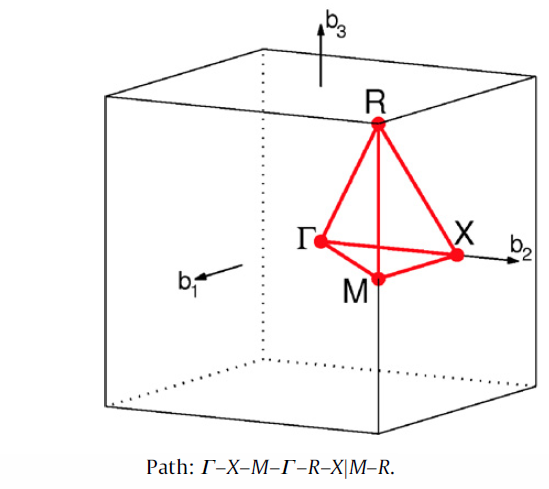
\includegraphics[height=2.10in,width=2.00in,viewport=90 0 550 500,clip]{Figures/Brillouin-Zone_CUB.png}}
\subfigure[\textrm{Band Structure of SrSnO$_3$}]{
\label{Band_Gap_SrSnO3}
\vspace*{-0.50in}
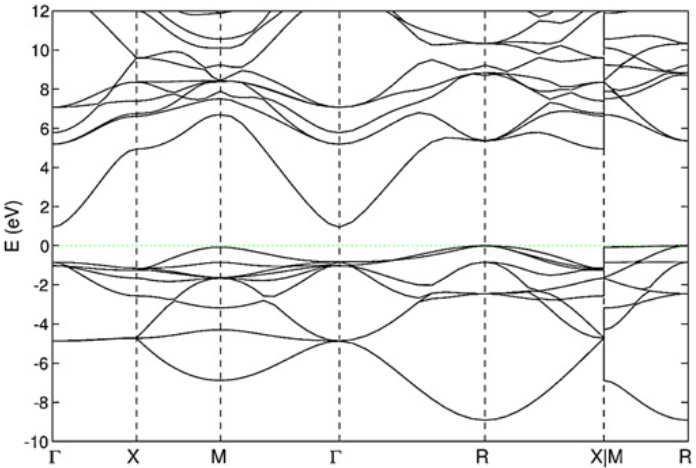
\includegraphics[height=2.10in,width=1.95in,viewport=0 0 710 550,clip]{Figures/Band-Struct_SrSnO3.png}}
\label{Band_Gap_CUB_SrSnO3}
\end{figure}
在固体能带理论中,能量色散关系$\varepsilon(\vec k)$~表示能量在倒空间中分布,其中量子数$\vec k$~(晶体动量)描述平移对称性
%\textcolor{blue}{能带图表示能量在\textrm{Brillouin-zone~}特定方向的色散关系}
}

\frame
{
	\frametitle{$\vec k$~空间布点与\textrm{Fermi~}面的确定}
\begin{figure}[h!]
\centering
%\hspace*{-10pt}
\vspace*{-0.3in}
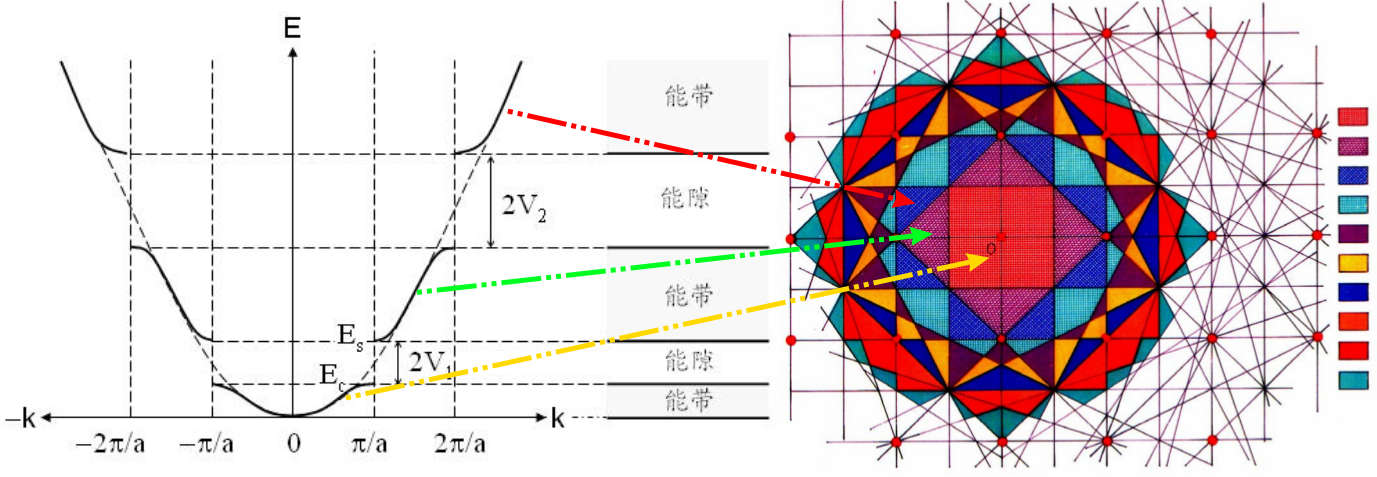
\includegraphics[height=1.5in,width=4.1in,viewport=0 5 1400 500,clip]{Figures/Brillouin-Band.png}
\caption{\small \textrm{The relation between unfolded-Band and the Brillouin-zone.}}%
\label{Brillouin-Band}
\end{figure} 
周期体系的\textrm{Fermi~}能级和\textrm{Fermi~}面的确定:\\
\begin{dislaymath}
	\left\{
	\begin{aligned}
		&\mbox{\textcolor{red}{导体:~}}&\mbox{\textcolor{blue}{价电子在\textrm{Brillouin-zone~}部分填充}}\\
		&\mbox{\textcolor{red}{半导体-绝缘体:~}}&\mbox{\textcolor{blue}{价电子在\textrm{Brillouin-zone~}完全填充}}
	\end{aligned}\right.
\end{dislaymath}
}

\frame
{
	\frametitle{$\vec k$~空间布点与\textrm{Fermi~}面的确定}
\begin{figure}[h!]
\centering
%\hspace*{-10pt}
\vspace*{-0.3in}
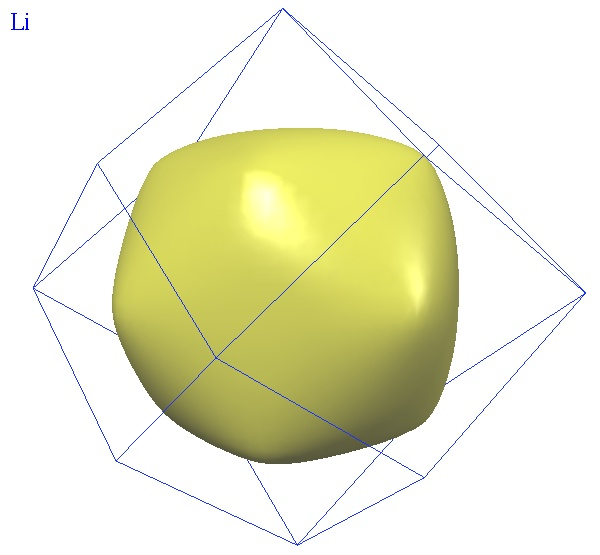
\includegraphics[height=1.3in,width=1.4in,viewport=0 0 110 100,clip]{Figures/FS-Li.jpg}
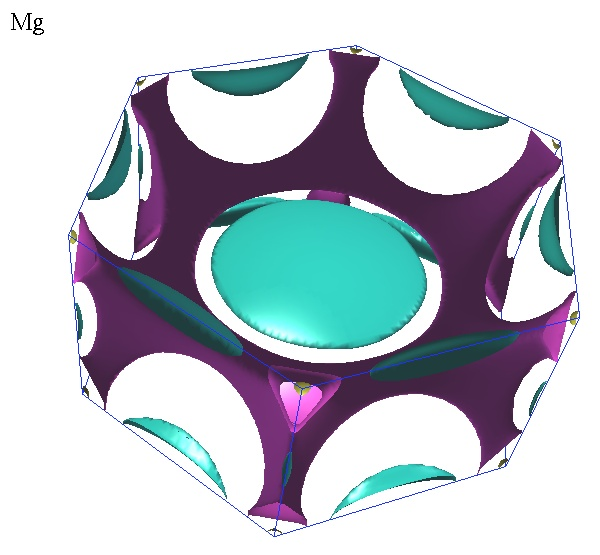
\includegraphics[height=1.3in,width=1.4in,viewport=0 0 110 100,clip]{Figures/FS-Mg.jpg}
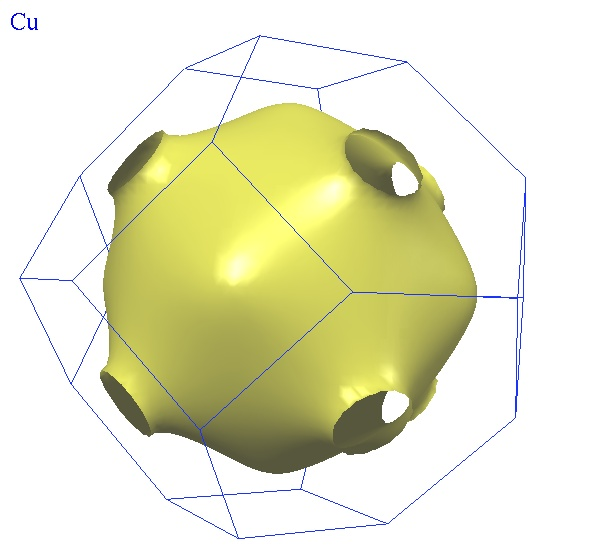
\includegraphics[height=1.3in,width=1.4in,viewport=0 0 110 100,clip]{Figures/FS-Cu.jpg}
\caption{\small \textrm{The Fermi-surface of Li, Mg, Cu in the first Brillouin-zone.}}%
\label{Brillouin-Band}
\end{figure} 
\textcolor{blue}{\textrm{Fermi~}面的形状}:\\
\textcolor{red}{最高占据能带折叠到第一\textrm{Brillouin-zone~}围成的区域}

\vspace{10pt}
要确定\textrm{Fermi~}面的精细结构,\underline{\textcolor{red}{特别是对于金属和导体体系}},必须在整个\textrm{Brillouin-zone~}取足够多的采样点
}

\frame
{
\frametitle{$\vec k$~空间积分与物理量}
与\textrm{Fermi~}面的确定类似,周期体系中所有单粒子期望值可表示为整个\textrm{Brillouin-zone~}内占据态的矩阵元的积分\\

一般地,如果已知\textrm{Brillouin-zone~}某点$\vec k$~的能带指标为$n$的波函数本征态$\Psi_n(\vec k)$~和本征值$\epsilon_n(\vec k)$,算符$\mathbf{X}$~的期望值$\langle X \rangle$是矩阵元
\begin{displaymath}
	X_n(\vec k)=\langle\Psi_n(\vec k)|\mathbf{X}|\Psi_n(\vec k)\rangle 
\end{displaymath}
\textcolor{blue}{在倒空间全部占据能带的求和}
\begin{displaymath}
	\langle X\rangle=\dfrac1{\sqrt V_G}\sum_n\int_{V_G}\mathrm{d}^3kX_n(\vec k)f(\varepsilon_n(\vec k))
\end{displaymath}
其中$V_G$是第一\textrm{Brillouin-zone}体积,$f(\varepsilon)$~是占据分布函数

实际计算中,\textrm{Brillouin-zone~}的$\vec k$~点数是有限的
\begin{displaymath}
	\langle X\rangle=\sum_{j,n}X_n(\vec k_j)w_n^{\vec k_j}
\end{displaymath} 
\textcolor{blue}{$\vec k$~点数目决定了电子结构和物理量的的精度与计算量}
}

\frame
{
\frametitle{$\vec k$~空间布点方案}
\begin{enumerate}
	\item \textcolor{red}{简单分布函数}\\
		\begin{itemize}
			\item 
				\begin{figure}[h!]
					\begin{minipage}[t]{0.40\linewidth}
						\textrm{Fermi-Dirac~}分布函数$$f(\varepsilon)=\dfrac1{\mathrm{e}^{(\varepsilon-\mu)/kT}+1}$$ 
						其中$\mu$是化学势,$k$~是\textrm{Boltzmann}常数,$T$是温度参数
					\end{minipage}
				\hfill
					\begin{minipage}[t]{0.55\linewidth}
					\centering
					\vspace*{-0.35in}
					\hspace*{-0.5in}
					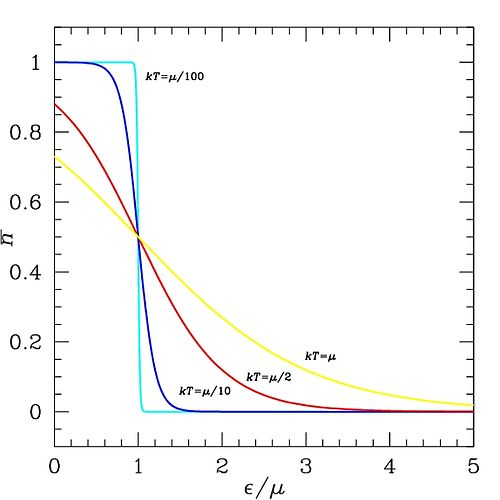
\includegraphics[height=1.0in,width=1.25in,viewport=0 0 530 500,clip]{Figures/Fermi-Dirac-distribution.jpg}
					\caption{\textrm{The Fermi-Dirac Distribution.}}%
					\label{Fermi-Dirac-distribution}
					\end{minipage}
					%\hspace*{-10pt}
				\end{figure} 
			\item 
				\begin{figure}[h!]
					\begin{minipage}[t]{0.40\linewidth}
						\textrm{Gaussian~}分布函数$$f(\varepsilon)=\dfrac1{\sigma\sqrt{2\pi}}\mathrm{e}^{-\frac{(\varepsilon-\mu)^2}{2\sigma^2}}$$
						其中$\mu$是化学势,$\sigma$是展宽参数
					\end{minipage}
				\hfill
					\begin{minipage}[t]{0.55\linewidth}
					\centering
					\vspace*{-0.35in}
					\hspace*{-0.5in}
					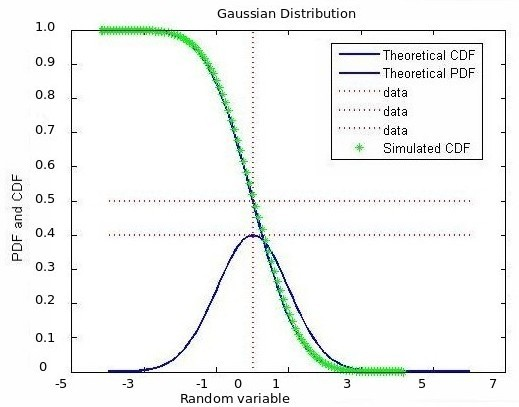
\includegraphics[height=1.0in,width=1.25in,viewport=0 0 530 500,clip]{Figures/Gaussian-distribution.jpg}
					\caption{\small \textrm{The Gaussian Distribution.}}%
					\label{Gaussian-distribution}
					\end{minipage}
					%\hspace*{-10pt}
				\end{figure} 
		\end{itemize}
\end{enumerate}
}

\frame
{
\frametitle{$\vec k$~空间布点方案}
\begin{enumerate}
	\setcounter{enumi}{1}
\setlength{\itemsep}{10pt}
	\item \textcolor{red}{特殊点方法\textrm{(Special-point scheme)}}\\这是一种相对高效的积分方法,通过选取少量有代表性的$\vec k$~点,即可获得较高的计算精度,这些$\vec k$~点被称为“平均值点”或“特殊点”\\特殊点方法对导体的收敛性较差
	\item \textcolor{red}{四面体方法\textrm{(Tetrahedron schemen)}}\\这是一种线性插值方法,将\textrm{Brillouin-zone~}用体积相等的四面体填充,在每个四面体内部,被积函数$X_n(\vec k_j)$和能量$\varepsilon_n^{\vec k_j}$都随$\vec k$~点线性变化\\一般来说,四面体方法对金属和导体的\textrm{Fermi~}面确定更可靠
\end{enumerate}
\textcolor{blue}{如何方便地确定每个$\vec k$~点的积分权重$w_n^{\vec k_i}$,精确、高效地完成\textrm{Brillouin-zone~}积分是$\vec k$~空间布点方案的主要研究内容}
}

\section{特殊点布点与积分方法}
\frame
{
	\frametitle{特殊点布点方案}
%如果采用一般的\textrm{Brillouin-zone~}内均匀选取$\vec k$~点的方法,为得到精确的结果,$\vec k$~点的密度必须非常大,从而导致计算量非常大,计算效率低下。因此需要寻求一种高效的积分方法。
	特殊点方法通过少量$\vec k$~点计算取得较高的精度,这些$\vec k$~点称为“平均值点”\upcite{PRB7-5212_1973}或“特殊点”\upcite{PRB8-5747_1973}。
	
	\textrm{Chadi}和\textrm{Cohen}最早提出特殊点方法的数学基础:\\
	考虑任意平滑函数$g(\vec k)$,可以展开为\textrm{Fourier}~级数之和
	$$g(\vec k)=f_0+\sum_{m=1}^{\infty}g_m\mathrm{e}^{\mathrm{i}\vec k\cdot\vec R_m}$$
\begin{figure}[h!]
\begin{minipage}[t]{0.55\linewidth}
	与$g(\vec k)$~对应的具有体系全部对称性的函数$f(\vec k)$,满足
	$$f(\mathbf{T}\vec k)=f(\vec k)\quad\forall\mathbf{T}\in\{\mathbf{G}\}$$
	因此可将$f(\vec k)$用$g(\vec k)$展开
	$$f(\vec k)=\dfrac1{n_{\mathbf{T}}}\sum\limits_ig(\mathbf{T}_i\vec k)$$
\end{minipage}
\hfill
\begin{minipage}[t]{0.42\linewidth}
\centering
\vspace*{-0.5in}
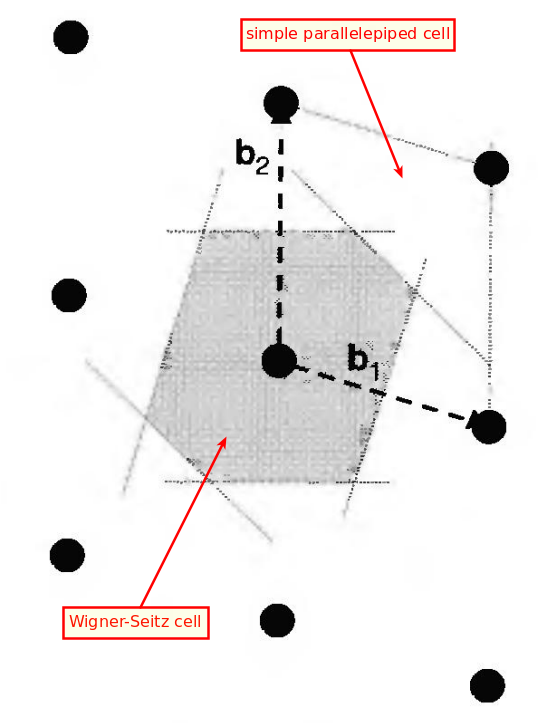
\includegraphics[height=1.8in,width=1.25in,viewport=20 20 530 800,clip]{Figures/Reciprocal-WS.png}
\caption{\small \textrm{The Wigner-Seitz Cell in the Brillouin-zone.}}%
\label{Reciprocal-WS}
\end{minipage}
%\hspace*{-10pt}
\end{figure} 
}

\frame
{
	\frametitle{特殊点布点方案}
	$f(\vec k)$可以写成
	$$f(\vec k)=f_0+\sum_{m=1}^{\infty}f_mA_m(\vec k)$$其中
	$$A_m(\vec k)=\sum_{|\vec R|=C_m}\mathrm{e}^{\mathrm{i}\vec k\cdot\vec R}\quad m=1,2,3,\cdots$$
	求和遍历所有对称操作群$\{\mathbf{T}\}$关联的等价矢量$\vec R$,因此$A_m(\vec k)$是实函数,满足
	\begin{displaymath}
		\begin{aligned}
			&\dfrac{V_G}{(2\pi)^3}\int_{\mathrm{BZ}}A_m(\vec k)\mathrm{d}\vec k=0\quad m=1,2,3,\cdots\\
			&\dfrac{V_G}{(2\pi)^3}\int_{\mathrm{BZ}}A_m(\vec k)A_n(\vec k)\mathrm{d}\vec k=N_n\delta_{nm}\quad m=1,2,3,\cdots\\
			&A_m(\mathbf{T}\vec k)=A_m(\vec k)
		\end{aligned}
	\end{displaymath}
}

\frame
{
	\frametitle{特殊点布点方案}
	令$A_0(\vec k)=1$,对函数$f(\vec k)$~在整个\textrm{Brillouin-zone}求平均有
	$$\bar f=\dfrac{V_G}{(2\pi)^3}\int_{\mathrm{BZ}}f(\vec k)\mathrm{d}\vec k=f_0$$
	同样地,函数$g(\vec k)$在\textrm{Brillouin-zone}的积分也是$f_0$

	结论:~\textcolor{red}{可通过选取优化的少量$\vec k$点求和计算平均值}\\如果存在一个$\vec k_0$点满足\textcolor{blue}{
	$$A_m(\vec k_0)=0\quad m=1,2,3,\dots,N$$}
	如果$N\rightarrow\infty$,则有$\bar f=f_0=f(\vec k_0)$精确成立,实际上这样的$\vec k_0$并不存在
\begin{figure}[h!]
\centering
%\hspace*{-10pt}
\vspace*{-0.2in}
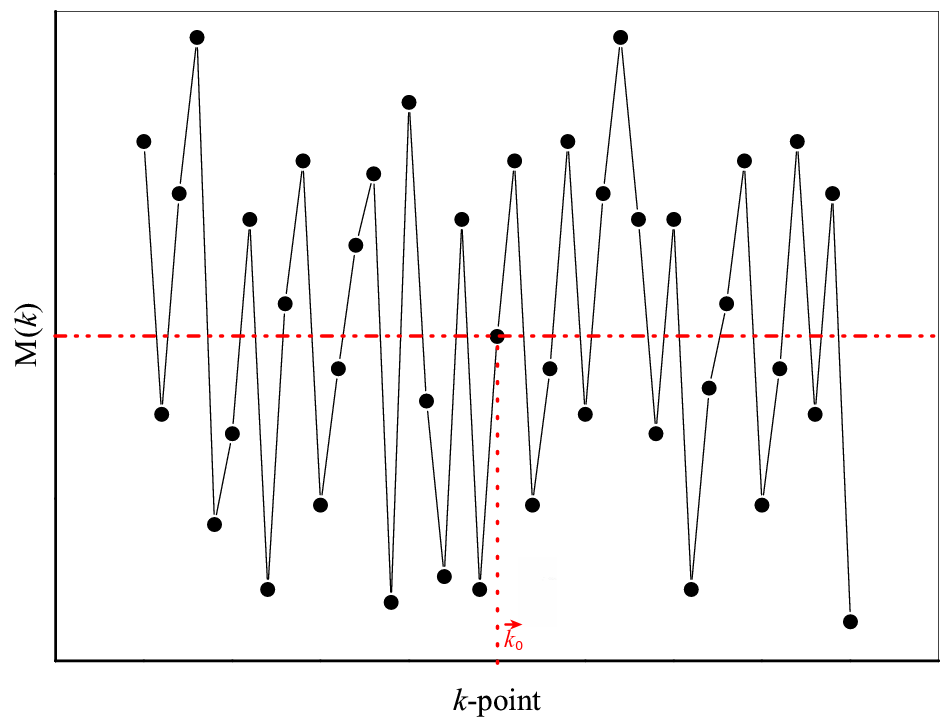
\includegraphics[height=1.1in,width=1.3in,viewport=5 0 960 750,clip]{Figures/Brillouin-k.png}
\caption{\small \textrm{The mean value and the $\vec k$-point.}}%
\label{Brillouin-k}
\end{figure} 
}

\frame
{
	\frametitle{特殊点布点方案}
	当$\vec k$-点数目$N$很大时,一般找到单个$\vec k_0$~点不容易,而选择满足一定条件的$\vec k$~点集合$\{\vec k\}$,利用这些$\vec k$~点加权平均计算$f_0$:\\
	假设有如下$\vec k_i$,权重为$\alpha_i$,并满足
	\begin{equation}
		\begin{aligned}
			&\sum_{i=1}^n\alpha_iA_m(\vec k_i)=0\quad m=1,2,3,\cdots,N\\
			&\sum_{i=1}^n\alpha_i=1
		\end{aligned}
		\label{eq:Chadi-Cohen}
	\end{equation}
	函数$f(\vec k)$在\textrm{Brillouin-zone}的积分值$f_0$可以表示为$$f_0\approx\sum_{i=1}^n\alpha_if(\vec k_i)$$
	\textcolor{blue}{对$\vec k$~点的选择,要求满足}
	\begin{enumerate}
		\item 集合$\{\vec k_i\}$中的$\vec k$~点数目尽可能少
		\item $\vec k_i$在$N$~尽可能大的条件下满足式\eqref{eq:Chadi-Cohen}
	\end{enumerate}
}

\frame
{
	\frametitle{\textrm{Chadi-Cohen}布点方案}
	\textrm{Chadi}和\textrm{Cohen}提出一套可以得到特殊$\vec k$~点的方法:
	\begin{itemize}
		\item \textcolor{blue}{确定两个特殊$\vec k$~点$\vec k_1$和$\vec k_2$}\\
		$\{N_1\}$(对应于$\vec k_1$)和$\{\vec N_2\}$(对应于$\vec k_2$)的情况下满足$$A_m(\vec k)=0$$
	\item \textcolor{blue}{由$\vec k_1$~和$\vec k_2$~确定一套新的$\vec k$~点集合}$$\vec k_i=\vec k_1+\mathbf{T}_i\vec k_2$$
			$\vec k_i$在条件$\vec k_i\in\{N_1\}\cup\{N_2\}$下仍然满足式\eqref{eq:Chadi-Cohen}
		\item \textcolor{blue}{确定$\vec k_i$的权重$\alpha_i$}
			$$\alpha_i=\dfrac{\alpha_i}{\sum\limits_jn_j}$$
	\end{itemize}
	重复上述过程,可以到一些列的特殊$\vec k$~点\\考虑体系对称性,集合$\{\vec k\}$~中的$\vec k$~点数目可以减少
}

\frame
{
	\frametitle{\textrm{Monkhorst-Pack}布点方案}
	\begin{itemize}
		\item \textrm{Chadi-Cohen}方案非常巧妙,但具体应用必须首先确定$2\sim3$个性能较好的$\vec k$~点,由此构建$\vec k$~点集合拥有比较高的效率和精度,所以每个具体体系,计算前必须经过相当的对称性分析。从程序编写角度来说,非常麻烦
		\item \textrm{Monkhorst-Pack}针对\textrm{Chadi-Cohen}方案提出一套简易的$\vec k$~点网格,并要求$\vec k$~点满足式\eqref{eq:Chadi-Cohen}:

\begin{figure}[h!]
\begin{minipage}[t]{0.55\linewidth}
			\textrm{Monkhorst-Pack}简易按如下方案划分\textrm{Brillouin-zone}:
			$$\boxed{u_r=\dfrac{(2r-q-1)}{2q}\quad(r=1,2,3,\cdots,q)}$$
			$q$是确定特殊点数目的某个整数
			\vspace{-0.1in}
			$$A_m(\vec k)=N_m^{-1/2}\sum_{|\vec R|=C_m}\mathrm{e}^{\mathrm{i}\vec k\cdot\vec R}$$
\end{minipage}
\hfill
\begin{minipage}[t]{0.42\linewidth}
\centering
%\hspace*{2pt}
\vspace*{-0.6in}
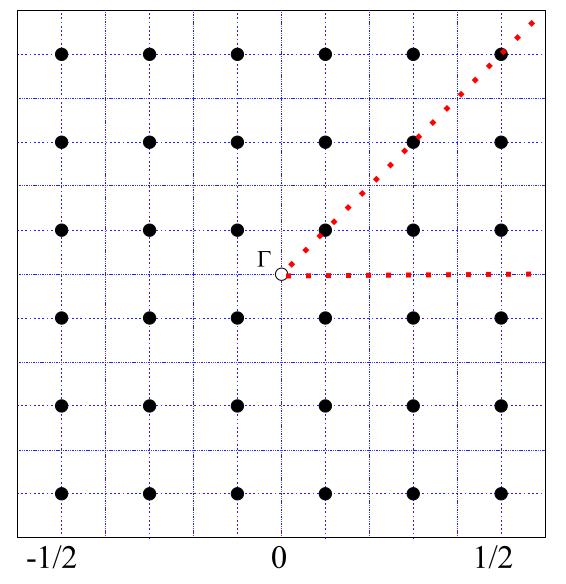
\includegraphics[height=1.5in,width=2.05in,viewport=-200 0 850 800,clip]{Figures/Special-points-MP.png}
\caption{\small \textrm{The generation of special $\vec k$-points in \textrm{Monkhorst-Pack} method.}}%
\label{Special-points-MP}
\end{minipage}
\end{figure} 
	\end{itemize}
}

\frame
{
	\frametitle{\textrm{Monkhorst-Pack}布点方案}
	对完全对称化函数$f(\vec k)$,用$A_m(\vec k)$展开
	$$f(\vec k)=\sum_{m=0}^{\infty}f_mA_m(\vec k)$$
	因为$A_m(\vec k)$在\textrm{Brillouin-zone}正交,可得
	$$f_m=\dfrac{V_G}{(2\pi)^3}\int_{\mathrm{BZ}}\mathrm{d}\vec kA_m^{\ast}(\vec k)f(\vec k)$$
	由此可得函数$f(\vec k)$~在\textrm{Brillouin-zone}积分
	$$\int_{\mathrm{BZ}}\mathrm{d}\vec kf(\vec k)=\dfrac{(2\pi)^2}{V_G}f_0$$
	\textcolor{blue}{可见\textrm{Monkhorst-Pack}方案与\textrm{Chadi-Cohen}方案是一致的}
}

\frame
{
	\frametitle{\textrm{Monkhorst-Pack}布点方案}
	考虑晶格点群对称性,%对$\vec k$~点数的求和可以变成不等价点$\vec k_j$~和每个$\vec k_j$~点的等价数的权重$w_j$求和表示\\
	如果$P(q)$是一套$\vec k$~点($\{\vec k_{prs}\}$)中不可约\textrm{Brillouin-zone}的$\vec k_j$~的对称性关联的等价点数,对$f_m$用一套离散的$\vec k_j$~点近似求和可以表示为
	$$\bar f_m=\dfrac1{q^3}\sum_{j=1}^{P(q)}w_j(q)f(\vec k_j)A_m(\vec k_j)$$
%	其中
%	$$w_j^{ab}=\dfrac1q\sum_{r=1}^q\mathrm{e}^{(\mathrm{i}\pi/q)(2r-q-1)(R_j^b-R_j^a)}$$
%	可有
%	\begin{displaymath}
%		W_j^{ab}(q)=\left\{
%		\begin{aligned}
%			&1 \qquad\qquad\mathrm{if}\, |R_j^b-R_j^a|=0,2q,4q,\cdots \\
%			&(-1)^{q+1}\quad \mathrm{if}\, |R_j^b-R_j^a|=q,3q,5q,\cdots \\
%			&0 \qquad\qquad\mathrm{otherwise}
%		\end{aligned}
%		\right.
%	\end{displaymath}
	由此得到$f(\vec k)$~的近似表达$\bar f(\vec k)$表示为
	$$\bar f(\vec k)=\sum_m\bar f_mA_m(\vec k)$$
	对$m$~的求和满足\textcolor{red}{布点约束条件}
	$$|R_j^a|<q/2,\,|R_j^b|<q/2\quad(j=1,2,3)$$
	其中$q$,$R_j^a$,$R_j^b$是整数
}

\frame
{
	\frametitle{\textrm{Monkhorst-Pack}布点的误差}
	\textrm{Monkhorst-Pack}\,布点积分的误差定义
	$$\epsilon_{\mathrm{BZ}}\equiv\int_{\mathrm{BZ}}\mathrm{d}\vec k[f(\vec k)-\bar f(\vec k)]=\sum_{m>1}f_mN_m^{1/2}S_{m1}(q)$$
	这里
	\begin{displaymath}
		S_{m1}(q)=\left\{
		\begin{aligned}
			&(-1)^{(q+1)(R_1+R_2+R_3)/q}\quad \mathrm{if}\; R_1-R_3\; \mathrm{are\, multiples\, of\, q} \\
			&\quad\qquad\qquad 0 \qquad\qquad\qquad \mathrm{otherwise}
		\end{aligned}
		\right.
	\end{displaymath}
	\textcolor{blue}{实际计算中,很多体系的积分与占据数有关,这样只有\textrm{Fermi}面包围的区域对积分有贡献}
	$$\int_{<\mathrm{FS}}\mathrm{d}\vec k f(\vec k)\approx\sum_m\bar f_mI_m(\vec k)$$
	其中
	$$I_m=\int_{<\mathrm{FS}}\mathrm{d}\vec k A_m(\vec k)$$
}

\frame
{
	\frametitle{\textrm{Monkhorst-Pack}布点的误差}
	因此,对\textrm{Fermi}面的积分误差是
	\begin{displaymath}
		\begin{aligned}
			\epsilon_{<\mathrm{FS}}&\equiv\int_{<\mathrm{FS}}\mathrm{d}\vec k[f(\vec k)-\bar f(\vec k)]\\
			&=\sum_m(f_m-\bar f_m)I_m+\sum_{m^{\prime}}f_{m^{\prime}}I_{m^{\prime}}
		\end{aligned}
	\end{displaymath}
	其中对$m^{\prime}$的求和表示求和部分不满足布点约束条件

	\begin{itemize}
		\item \textcolor{red}{当$\vec k_j$~求和遍历\textrm{Brillouin-zone}全部不可约区域,\textrm{Monkhorst-Pack}方法积分是精确和高效的}
		\item \textcolor{blue}{对于立方晶系,$q$~值尽量取为偶数}\\
			目的:~避免选择类似$\Gamma$~点这样的高对称性点,得到更合理的统计平均值
	\end{itemize}
}

%\frame
%{
%\begin{figure}[h!]
%\centering
%\vspace*{-0.25in}
%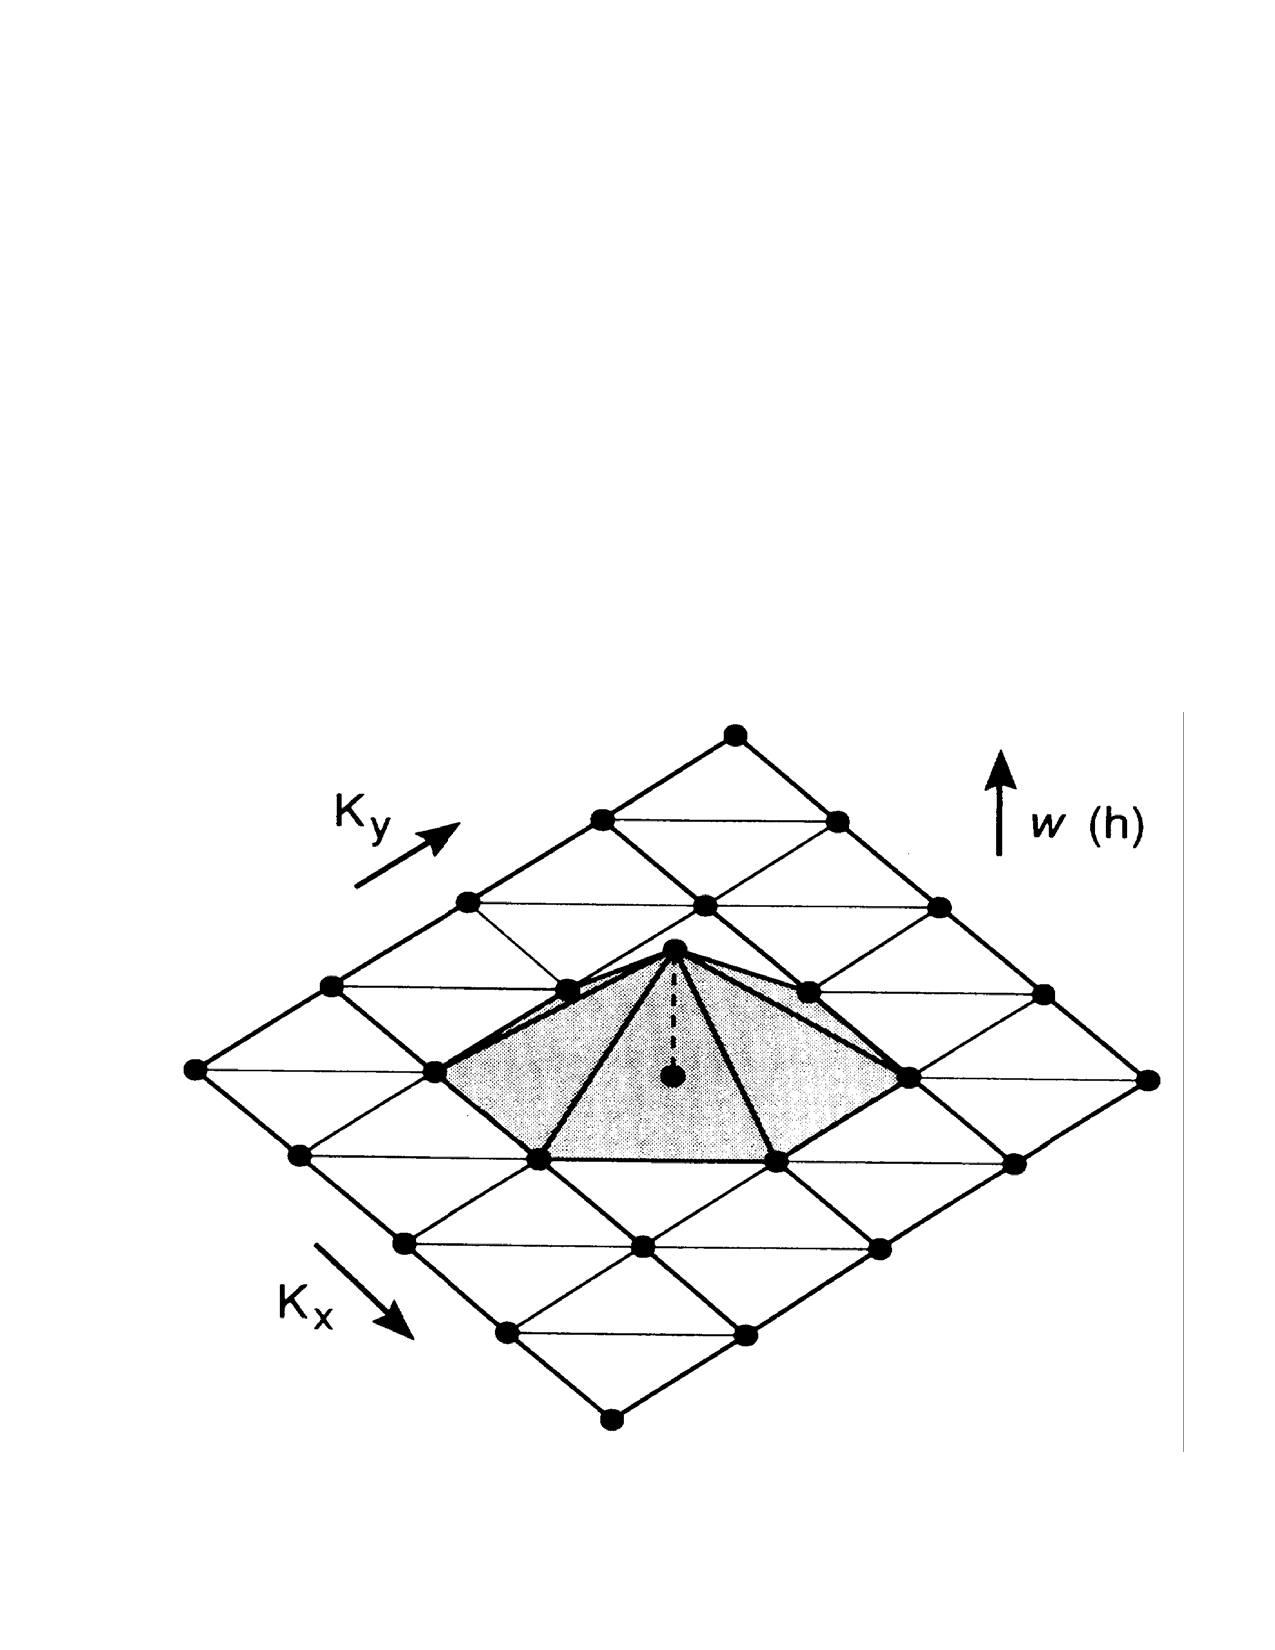
\includegraphics[height=2.75in,width=3.05in,viewport=0 30 565 505,clip]{Figures/dimen_Tetra.pdf}
%\caption{\small Two-dimensional schematic illustration of the function $w_j(\vec k)$.}%(与文献\cite{EPJB33-47_2003}图1对比)
%\label{Fig:Submesh_Tetra}
%\end{figure}
%}

\appendix
%------------------------------------------------------------------------Reference----------------------------------------------------------------------------------------------
%\begin{thebibliography}{99}
%-----------------------------------------------------------------------------------------------------------------------------------------------------------------------%
%\frame
%{
%\frametitle{主要参考文献}
%{\small
%\bibitem{Singh_Book}\textrm{D. J. Singh. \textit{Plane Wave, PseudoPotential and the LAPW method} (Kluwer Academic, Boston,USA, 1994)}					%
%  \nocite{*}																				%
%}
%}
%\end{thebibliography}

\begin{thebibliography}{99}
\frame
{
\frametitle{主要参考文献}
{\small
%	\bibitem{Huang_Han}黄昆\:原著、韩汝琦\:改编, {\textit{固体物理学}}\:高等教育出版社, 北京, 1988
%	\bibitem{Xie_Lu}谢希德、陆栋\:主编, {\textit{固体能带理论}}\:复旦大学出版社, 上海, 1998
	\bibitem{PRB7-5212_1973}\textrm{A. Baldereschi \textit{Phys. Rev.} B, \textbf{7} (1973), 5212}
	\bibitem{PRB8-5747_1973}\textrm{D. J. Chadi and M. L. Cohen \textit{Phys. Rev.} B, \textbf{8} (1973), 5747}
	\bibitem{PRB13-5188_1976}\textrm{H. J. Monkhorst and J. D. Pack \textit{Phys. Rev.} B, \textbf{13} (1976), 5188}
        \bibitem{Singh_Book}\textrm{D. J. Singh. \textit{Plane Wave, PseudoPotential and the LAPW method} (Kluwer Academic, Boston,USA, 1994)}
}
\nocite*{}
}
\end{thebibliography}
%{\small
%\phantomsection\addcontentsline{toc}{section}{Bibliography}	 %直接调用\addcontentsline命令可能导致超链指向不准确,一般需要在之前调用一次\phantomsection命令加以修正	%
%\bibliography{Myref}																			%
%\bibliographystyle{mybib}																		%
%  \nocite{*}																				%
%}
%-----------------------------------------------------------------------------------------------------------------------------------------------------------------------%


%-----------------------------------------------------------Beamer下不建议使用bib,因为涉及分页--------------------------------------------------------------------------%
%{\small
%\phantomsection\addcontentsline{toc}{section}{Bibliography}	 %直接调用\addcontentsline命令可能导致超链指向不准确,一般需要在之前调用一次\phantomsection命令加以修正	%
%\bibliography{Myref}																			%
%\bibliographystyle{mybib}																		%
%  \nocite{*}																				%
%}

%------------------------------------------------------------------------------------------------------------------------------------------------------------------------------%

%-------------------------------------------------------------------------Thanks------------------------------------------------------------------------------------------------
%\section{致谢}
%\frame
%{
%\frametitle{致$\quad$谢}
%\begin{itemize}
%    \setlength{\itemsep}{20pt}
%  \item 感谢本团队高兴誉、吴泉生、宋红州等各位老师参与的讨论
%  \item 感谢莫所长、宋主任以及软件中心各位老师和同事
%  \item 感谢王崇愚先生的帮助
%\end{itemize}
%}

\logo{}									%不显示logo
\frame
{
\vskip 60 pt
%\hskip 10pt \textcolor{blue}{\Huge 感谢答辩委员会各位老师\,\textrm{!}}\\
\vskip 35 pt
\hskip 60pt \textcolor{blue}{\Huge 谢谢大家\:!}
%\vskip 15 pt
%\hskip 40pt \textcolor{blue}{\Huge \textrm{for your attention\:!}}
}

%-------------------------------------------------------------------------------------------------------------------------------------------------------------------------------

\clearpage
%\end{CJK*}
\end{document}
